\documentclass[12pt,letterpaper]{article}
\usepackage{fullpage}
\usepackage{wrapfig}
\usepackage{graphicx}
\usepackage{fancyhdr,lastpage}
\usepackage{amsmath,amssymb}
\usepackage{color}

% some formatting from http://www.tedpavlic.com/post_homework_tex_example.php:
% In case you need to adjust margins:
\topmargin=-0.45in      %
\evensidemargin=0in     %
\oddsidemargin=0in      %
\textwidth=6.5in        %
\textheight=9.0in       %
\headsep=0.25in         %
\headheight=30pt

\newcommand{\probnumber}[1]{\vspace{2em}\noindent\textbf{(#1)}}

\newcommand{\SE}{{\mbox{SE}}}
\newcommand{\ch}[2]{{{}_{#1}C_{#2}}}
\newcommand{\prob}{{\mbox{Pr}}}
\newcommand{\wt}{\widetilde}
\renewcommand{\SS}{{\mbox{SS}}}
\newcommand{\MS}{{\mbox{MS}}}
\newcommand{\df}{{\mbox{df}}}
\renewcommand{\P}{\mathbb{P}}


\newif{\ifanswers}
\answerstrue
% \answersfalse

\newcommand{\answer}[1]{{\ifanswers {\color{red}\textsf{#1}} \else {} \fi}}

\begin{document}


Write the name of an appropriate statistical procedure --
for instance ``Wilcoxon--Mann--Whitney test'' or ``chi-squared for goodness of fit'' or ``$t$-test for difference in means''.
\begin{enumerate}
        \renewcommand{\theenumi}{\textbf{\Alph{enumi}}}

    \item We have measured the average flying speeds in five groups of 20 flies;
        each group was given a different number of milligrams of caffeine in their food.
        How much does the average flying speed increase, per milligram of caffeine?
        
        \answer{$t$-test for no linear correlation/$r=0$/slope $b_1=0$}
      \ifanswers \else \vspace{3\baselineskip} \fi

    \item 
        We have measured heart rates in patients given combinations of dosages
        of two different drugs (none, low, and high doses for each, for a total of nine combinations).
        Is there an interaction between the drugs?
        
        \answer{$F$-test for two-way ANOVA, for interactions}
      \ifanswers \else \vspace{3\baselineskip} \fi

    \item 
        We have surveyed 100 randomly chosen individuals in Los Angeles and in Pasadena,
        and determined if they had a hospital visit in the last year.
        Does this differ between cities?
        
        \answer{chi-squared test for a $2 \times 2$ contingency table}
      \ifanswers \else \vspace{3\baselineskip} \fi


\end{enumerate}



\hrule
\vspace{3em}



% numerical data in categories
% find SS, MS
% do F-test for mean effects
% interpret
To study whether summer daylength causes human hair to absorb more light,
we measured hair absorbance (larger numbers mean more absorbance) in random samples from four cities at different latitudes in Europe, summarized here:
\begin{center}
\begin{tabular}{lrrrr}
  \hline
 & Barcelona & London & Paris & Stockholm \\ 
  \hline
mean & 4.41 & 5.04 & 4.73 & 5.52 \\ 
  SD & 0.84 & 0.71 & 0.90 & 0.87 \\ 
  n & 12 & 10 & 20 & 9 \\ 
   \hline
\end{tabular}
\end{center}

\begin{enumerate}
        \renewcommand{\theenumi}{\textbf{\Alph{enumi}}}
  \item State the null hypothesis in words, and then in symbols.

    \answer{
    \begin{align*}
      H_0 &: 
      \text{mean hair absorbance is the same in all cities} \\
&\mu_{\text{Barcelona}} = \mu_{\text{London}} = \mu_{\text{Paris}} = \mu_{\text{Stockholm}} \\
    \end{align*}
    }
    % \vspace{7\baselineskip}

  \item Construct the ANOVA table and test the null hypothesis.

    \answer{
        \emph{Note: I will not make you calculate the $\SS(\text{between})$, as we do below, on the test.}
    \begin{align*}
      \bar{\bar y} &= \frac{ 12 \times 4.41 +  10 \times 5.04 + 20 \times 4.73 + 9 \times 5.52 }{ 51 } = 4.854902 \\
      \SS(\text{within}) &= 11 \times 0.84^2 + 9 \times 0.71^2 + 19 \times0.90^2 + 8 \times 0.87^2 = 27.80723 \\
      \df(\text{within}) &= 47 \\
      \MS(\text{within}) &= 0.5916432 \\
      \SS(\text{between}) &= 12 \times (4.41-4.85)^2 + 10 \times (5.04-4.85)^2 + 20 \times (4.73-4.85)^2 + 9 \times (5.52-4.85)^2 \\
            &= 0.6901548 \\
      \df(\text{between}) &= 3 \\
      \MS(\text{between}) &= 0.2300516
    \end{align*}
    $F_s = 0.2300516/0.5916432 = 0.388835$, so $P>.2$.
    Fail to reject $H_0$.
    }
    % \vspace{7\baselineskip}

  \item Estimate the within-group variability with the pooled standard deviation.

    \answer{
    \[
    s_\text{pooled} = \sqrt{ \frac{ 11 \times 0.84^2 + 9 \times 0.71^2 + 19 \times .9^2 + 8 \times .87^2  }{ 47 } } = 0.8473199 ,
    \]
    }
    % \vspace{7\baselineskip}

  \item Assess the strength of the evidence for and against the alternative hypothesis (i.e.\ what can we conclude).

  \answer{
  We didn't find any evidence of a relationship between latitude and hair absorbance;
  however, there are confounding factors (genetics).
  Since the effect size we see is comparable to the within-group variability,
  we'd need much larger sample sizes, in any case.
  }

\end{enumerate}

\pagebreak

% bivariate continuous data, explicit
% formulate hypothesis
% do linear regression
% test for significant effect
\begin{wrapfigure}[8]{r}{2.5in}
  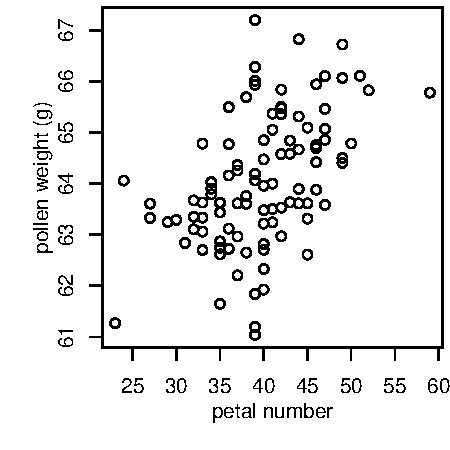
\includegraphics{sunflowers.pdf}
  \vspace{4in}
\end{wrapfigure}

It is hypothesized that flowers with more petals also produce more pollen.
To test this, we have measured petal number and weight of pollen of 100 sunflowers,
each from different plants,
shown at right.
The mean number of petals is 39.62, with an SD of 6.18;
the mean weight of pollen is 64.05, with an SD of 1.29;
and the correlation between them is $r=0.49$.

\vspace{1.4in}

{\color{white}a}

\begin{enumerate}
        \renewcommand{\theenumi}{\textbf{\Alph{enumi}}}
  \item Write the equation for the least-squares regression line,
      and draw this line on the plot.

      \answer{
      Slope is $b_1 = .49 \times 1.29 / 6.18 = 0.1022816$; intercept is $b_0 = 64.05-0.1022816\times39.62 = 59.9976$.
      \[
      \text{(pollen weight)} = 0.10 \times \text{(petal number)} + 60.0 .
      \]
      }
    % \vspace{6\baselineskip}

  \item Formulate null and alternative hypotheses appropriate for a test of a linear relationship in words, and then in symbols.

    \answer{
    \begin{align*}
      H_0 &: \text{there is not a linear relationship between average petal number and average pollen weight} \\
      & b_1 = 0 \\
      H_A &: \text{there is a linear relationship between average petal number and average pollen weight} \\
      & b_1 \neq 0 
    \end{align*}
    }
    % \vspace{5\baselineskip}

  \item Test the null hypothesis, and briefly state the conclusions.

    \answer{
      \begin{align*}
        t_s &= .49 \sqrt{ \frac{ 98 }{ 1-.49^2 } } = 5.564561 \\
        df &= 98
      \end{align*}
      and $P<.001$;
      we have strong evidence of a linear relationship between mean petal number and mean pollen weight.
    }
    % \vspace{7\baselineskip}

  \item If we found out that our field assistants had cut corners by collecting many of the sunflowers from the same plant, 
      would this call our conclusions into question? 
      Explain, briefly.

      \answer{
      Yes, because the samples are not independent (flowers from the same plant could be correlated), so we might be overly confident in our results.
      }
\end{enumerate}


\end{document}
